
%!TEX root = ../thesis.tex
%*******************************************************************************
%****************************** Second Chapter *********************************
%*******************************************************************************

\newcommand{\ba}{\mathbf{a}}
\newcommand{\bb}{\mathbf{b}}
\newcommand{\bd}{\mathbf{d}}
\newcommand{\bw}{\mathbf{w}}
\newcommand{\bx}{\mathbf{x}}
\newcommand{\by}{\mathbf{y}}
\newcommand{\Exp}[2]{\mathbb{E}_{#1}\left[#2\right]}
\newcommand{\Var}[2]{\text{Var}_{#1}\left[#2\right]}
\newcommand{\Cov}[2]{\text{Cov}_{#1}\left[#2\right]}
\newcommand{\Corr}[2]{\text{Corr}_{#1}\left[#2\right]}

\newcommand{\bA}{\mathbf{A}}
\newcommand{\bB}{\mathbf{B}}
\newcommand{\bV}{\mathbf{V}}
\newcommand{\bW}{\mathbf{W}}
\newcommand{\bv}{\mathbf{v}}

\newcommand{\bphi}{\mathbf{\phi}}
\newcommand{\bt}{\mathbf{\theta}}
\newcommand{\bdelta}{\mathbf{\delta}}
\newcommand{\beps}{\mathbf{\epsilon}}
\newcommand{\q}{q_\mathbf{\phi}}
\newcommand{\bmu}{\mathbf{\mu}}
\newcommand{\bsigma}{\mathbf{\sigma}}
\newcommand{\bSigma}{\mathbf{\Sigma}}

\newcommand{\D}{\mathcal{D}}

\newcommand{\eqnr}{\addtocounter{equation}{1}\tag{\theequation}}

\chapter{Background}

\ifpdf
    \graphicspath{{Chapter2/Figs/Raster/}{Chapter2/Figs/PDF/}{Chapter2/Figs/}}
\else
    \graphicspath{{Chapter2/Figs/Vector/}{Chapter2/Figs/}}
\fi


\fbox{
    \parbox{\textwidth}
    {
       Chapter Overview
        \begin{itemize}
            \item Neural Networks and Convolutional Neural Networks.
            \item Concepts like Variational Inference, and local reparameterization trick in Bayesian Neural Network.
            \item Backpropagation in Bayesian Networks using Bayes by Backprop.
            \item Estimation of Uncertainities in a network.
            \item Pruning a network to reduce the parameters without affecting the performance.
        \end{itemize}
    }
}

\pagebreak

\section{Neural Networks}
\subsection{Brain Analogies}

A perceptron is conceived as a mathematical model of how the neurons function in our brain by a famous psychologist Rosenblatt. According to him, a neuron  takes a set of binary inputs (nearby neurons), multiplies each input by a continuous valued weight (the synapse strength to each nearby neuron), and thresholds the sum of these weighted inputs to output a 1 if the sum is big enough and otherwise a 0 (in the same way neurons either fire or do not).

\begin{figure}[H]
\begin{center}
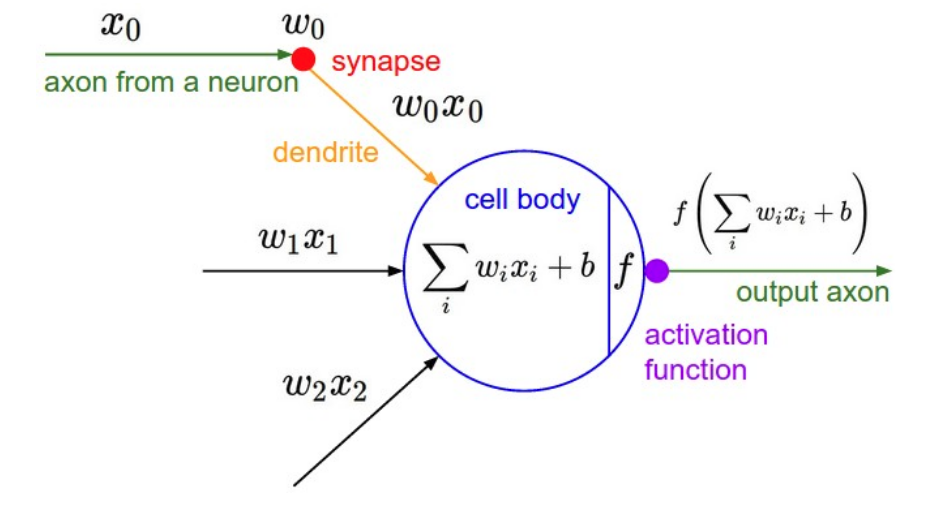
\includegraphics[height=.28\textheight]{Chapter2/Figs/NeuralNetwork.png}
\label{fig:Neural_Network}
\caption{Biologically inspired Neural Network \cite{karparthy}}
\end{center}
\end{figure}

\subsection{Neural Network}

Inspired from the biological nervous system, the structure of an Artificial Neural Network (ANN) is developed to process information similar to how brain process information. A large number of highly interconnected processing elements (neurons) working together makes a Neural Network to solve complex problems. Just like humans learn by example, so does a Neural Network. Learning in biological systems involves adjustments to the synaptic connections which is similar to weight updates in a Neural Network. 

A Neural Network consists of three layers : input layer to feed the data to the model to learn representation, hidden layer that learns the representation and the output layer that outputs the results or predictions. Neural Networks can be thought of an end to end system that finds patterns in data which are too complex to be recognized by a human to teach to a machine. 


\begin{figure}[H]
\begin{center}
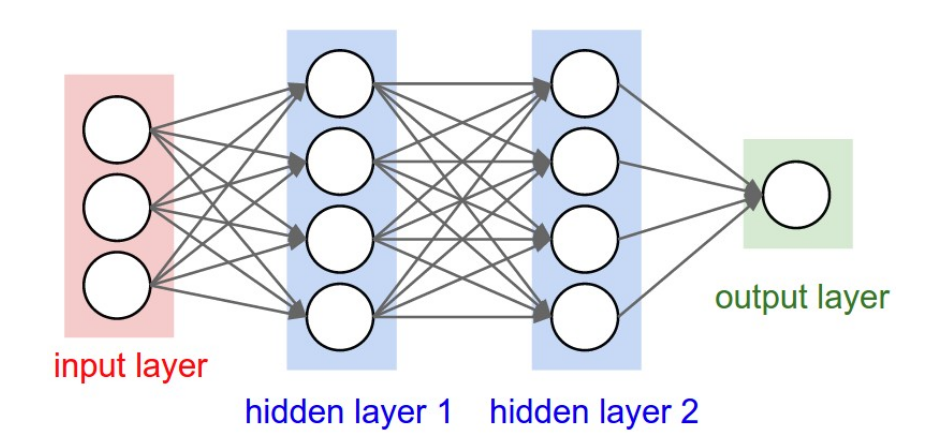
\includegraphics[height=.28\textheight]{Chapter2/Figs/TwoLayeredNN.png}
\label{fig:Two Layered Neural_Network}
\caption{Neural Network with two hidden layers \cite{karparthy}}
\end{center}
\end{figure}


\subsection{Convolutional Neural Network}

Hubel and Wiesel in their hierarchy model mentioned a neural network to have a hierarchy structure in the visual cortex. LGB (lateral geniculate body) forms the simple cells that forms the complex cells which forms the lower order hypercomplex cells that finally forms the higher order hypercomplex cells.
Also, the neural network between lower order hypercomplex cells and higher order hypercomplex cells are structurally similar to the network between simple cells and complex cells. In this hierarchy, a cell in a higher stage generally has a tendency to respond selectively to a more complicated feature of the stimulus pattern, and the cell at the lower stage responds to simpler features. Also, higher stage cells possess a larger receptive field, and is more insensitive to the shift in position of the stimulus pattern.

Similar to a hierarchy model, a neural network starting layers learns simpler features like edges and corners and subsequent layers learns complex features like colors, textures and so on. Unlike in multi layer perceptron where all neurons from one layer is connected with all the neurons in the next layer, weight sharing is the main idea behind a convolutional neural network. 
Example: instead of each neuron having a different weight for each pixel of the input image (28*28 weights), the neurons only have a small set of weights (5x5=25) that is applied a whole bunch of small subsets of the image of the same size. Layers past the first work in a similar way, but take in the ‘local’ features found in the previous hidden layer rather than pixel images, and so ‘see’ successively larger portions of the image since they are combining information about increasingly larger subsets of the image. Finally, the final layer makes the correct prediction for the output class.

The reason for why this is helpful is intuitively if not mathematically clear: without such constraints the network would have to learn the same simple things (such as detecting edges, corners, etc) a whole bunch of times for each portion of the image. But with the constraint there, only one neuron would need to learn each simple feature - and with far fewer weights overall, it could do so much faster! Moreover, since the pixel-exact locations of such features do not matter the neuron could basically skip neighboring subsets of the image - subsampling, now known as a type of pooling - when applying the weights, further reducing the training time. The addition of these two types of layers - convolutional and pooling layers - are the primary distinctions of Convolutional Neural Nets (CNNs/ConvNets) from plain old neural nets.


\section{Probabilistic Machine Learning}
\subsection{Variational Inference}

We define a function $y = f(\mathbf{x})$ that estimates the given inputs $\{ x_1, \hdots, x_N \}$ and their corresponding outputs $\{y_1, \hdots, y_N\}$ and produces an output. Using Bayesian inference, a prior distribution is used over the space of functions $p(f)$. This distribution represents our prior belief as to which functions are likely to have generated our data. 

A likelihood is defined as $p(Y | f, X)$ to capture the process in which given a function observation is generated. We use the Bayes rule to find the posterior distribution given our dataset : $p(f | X, Y)$.

The new output can be predicted for a new input point $x^*$ by integrating over all possible functions $f$,
\begin{align} \label{eq:post}
%p(\f | \X, \Y) \propto p(\Y | \X, \f) p(\f).
p(y^* | x^*, X, Y) = \int p(y^* | f^*) p(f^* | x^*, X, Y) df^*
\end{align}

The \eqref{eq:post} is intractable due to the integration sign. We can approximate it by taking a finite set of random variables $w$ and conditioning the model on it. However, it is based on a modelling assumption that the model depends on these variables alone, and making them into sufficient statistics in our approximate model.

The predictive distribution for a new input point $x^*$ is then given by 
$$
p(y^* | x^*, X, Y) = \int p(y^* | f^*) p(f^* | x^*, w) p(w | X, Y) df^* d w.
$$

However, the distribution $p(w | X, Y)$ still remains intractable and we need to approximate it with a variational distribution $q(w)$, that can be computed. The approximate distribution needs to be as close as possible to the posterior distribution obtained from the original model. We thus minimise the Kullback--Leibler (KL) divergence, intuitively a measure of similarity between two distributions: $KL(q(w) ~||~ p(w | X, Y))$,
resulting in the approximate predictive distribution 
\begin{align} \label{eq:predictive}
q(y^* | x^*) = \int p(y^* | f^*) p(f^* | x^*, w) q(w)  df^* dw.
\end{align}

Minimising the Kullback--Leibler divergence is equivalent to maximising the \textit{log evidence lower bound},
\begin{align}
KL_{\text{VI}} := \int q(w) p(F | X, w) \log p(Y | F) dF dw - \KL(q(w) || p(w)) \label{eq:L:VI}
\end{align}
with respect to the variational parameters defining $q(w)$. This is known as \textit{variational inference}, a standard technique in Bayesian modelling.

Maximizing the KL divergence between the posterior and the prior over $w$ will result in a variational distribution that learns a well representation from the data (obtained from log likelihood) and is closer to the prior distribution. In other words, it can prevent overfitting. 


\subsection{Local  reparametrisation  trick}

We therefore propose an alternative estimator for which we have $\Cov{}{L_{i},L_{j}} = 0$, so that the variance of our stochastic gradients scales as $1/M$. We then make this new estimator computationally efficient by not sampling $\beps$ directly, but only sampling the intermediate variables $f(\beps)$ through which $\beps$ influences $L_\D^\text{SGVB}(\bphi)$. By doing so, the global uncertainty in the weights is translated into a form of local uncertainty that is independent across examples and easier to sample. We refer to such a reparameterization from global noise to local noise as the \emph{local reparameterization trick}. Whenever a source of global noise can be translated to local noise in the intermediate states of computation ($\beps \rightarrow f(\beps)$), a local reparameterization can be applied to yield a computationally and statistically efficient gradient estimator.

Such local reparameterization applies to a fairly large family of models, but is best explained through a simple example: Consider a standard fully connected neural network containing a hidden layer consisting of 1000 neurons. This layer receives an $M \times 1000$ input feature matrix $\bA$ from the layer below, which is multiplied by a $1000 \times 1000$ weight matrix $\bW$, before a nonlinearity is applied, i.e. $\bB = \bA\bW$. We then specify the posterior approximation on the weights to be a fully factorized Gaussian, i.e.\ $\q(w_{i,j}) = N(\mu_{i,j},\sigma^{2}_{i,j}) \hspace{0.1cm} \forall w_{i,j} \in \bW$, which means the weights are sampled as $w_{i,j} = \mu_{i,j} + \sigma_{i,j}\epsilon_{i,j}$, with $\epsilon_{i,j} \sim N(0,1)$. In this case we could make sure that $\Cov{}{L_{i},L_{j}} = 0$ by sampling a separate weight matrix $\bW$ for each example in the minibatch, but this is not computationally efficient: we would need to sample $M$ million random numbers for just a single layer of the neural network. Even if this could be done efficiently, the computation following this step would become much harder: Where we originally performed a simple matrix-matrix product of the form $\bB = \bA\bW$, this now turns into $M$ separate local vector-matrix products. The theoretical complexity of this computation is higher, but, more importantly, such a computation can usually not be performed in parallel using fast device-optimized BLAS (Basic Linear Algebra Subprograms). This also happens with other neural network architectures such as convolutional neural networks, where optimized libraries for convolution cannot deal with separate filter matrices per example.

Fortunately, the weights (and therefore $\beps$) only influence the expected log likelihood through the neuron activations $\bB$, which are of much lower dimension. If we can therefore sample the random activations $\bB$ directly, without sampling $\bW$ or $\beps$, we may obtain an efficient Monte Carlo estimator at a much lower cost. For a factorized Gaussian posterior on the weights, the posterior for the activations (conditional on the input $\bA$) is also factorized Gaussian:
\begin{align}
\q(w_{i,j}) &= N(\mu_{i,j},\sigma^{2}_{i,j}) \hspace{0.1cm} \forall w_{i,j} \in \bW \hspace{0.2cm} \Longrightarrow \hspace{0.2cm} \q(b_{m,j}|\bA) = N(\gamma_{m,j},\delta_{m,j}), \text{ with } \nonumber\\
\gamma_{m,j} &= \sum_{i=1}^{1000} a_{m,i}\mu_{i,j}, \hspace{0.2cm} \text{ and } \hspace{0.2cm} \delta_{m,j} = \sum_{i=1}^{1000} a^{2}_{m,i}\sigma^{2}_{i,j}.
\end{align}
Rather than sampling the Gaussian weights and then computing the resulting activations, we may thus sample the activations from their implied Gaussian distribution directly, using $b_{m,j} = \gamma_{m,j} + \sqrt{\delta_{m,j}}\zeta_{m,j}$, with $\zeta_{m,j} \sim N(0,1)$. Here, $\zeta$ is an $M \times 1000$ matrix, so we only need to sample $M$ thousand random variables instead of $M$ million: a thousand fold savings.

In addition to yielding a gradient estimator that is more \textit{computationally efficient} than drawing separate weight matrices for each training example, the local reparameterization trick also leads to an estimator that has \textit{lower variance}. To see why, consider the stochastic gradient estimate with respect to the posterior parameter $\sigma^{2}_{i,j}$ for a minibatch of size $M=1$. Drawing random weights $\bW$, we get
\begin{align}
\label{eq:stochest_weights}
\frac{\partial L_\D^\text{SGVB}}{\partial \sigma^{2}_{i,j}} = \frac{\partial L_\D^\text{SGVB}}{\partial b_{m,j}}\frac{\epsilon_{i,j}a_{m,i}}{2\sigma_{i,j}}.
\end{align}
If, on the other hand, we form the same gradient using the local reparameterization trick, we get
\begin{align}
\label{eq:stochest_local}
\frac{\partial L_\D^\text{SGVB}}{\partial \sigma^{2}_{i,j}} = \frac{\partial L_\D^\text{SGVB}}{\partial b_{m,j}}\frac{\zeta_{m,j}a_{m,i}^{2}}{2\sqrt{\delta_{m,j}}}.
\end{align}
Here, there are two stochastic terms: The first is the backpropagated gradient $\partial L_{\D}^\text{SGVB} / \partial b_{m,j}$, and the second is the sampled random noise ($\epsilon_{i,j}$ or $\zeta_{m,j}$). Estimating the gradient with respect to $\sigma^{2}_{i,j}$ then basically comes down to estimating the covariance between these two terms. This is much easier to do for $\zeta_{m,j}$ as there are much fewer of these: individually they have higher correlation with the backpropagated gradient $\partial L_\D^\text{SGVB}/\partial b_{m,j}$, so the covariance is easier to estimate. In other words, measuring the effect of $\zeta_{m,j}$ on $\partial L_\D^\text{SGVB}/\partial b_{m,j}$ is easy as $\zeta_{m,j}$ is the only random variable directly influencing this gradient via $b_{m,j}$. On the other hand, when sampling random weights, there are a thousand $\epsilon_{i,j}$ influencing each gradient term, so their individual effects get lost in the noise. In appendix \ref{sec:low_variance_reparam} we make this argument more rigorous, and in section~\ref{sec:experiments} we show that it holds experimentally.


%The problem of approximating the gradient thus boils down to estimating one of the correlation coefficients $\rho_{1} = \Corr{q,\D}{\partial L_\D^\text{SGVB}/\partial b_{m,j}, \epsilon_{i,j}}$ or $\rho_{2} = \Corr{q,\D}{\partial L_\D^\text{SGVB}/\partial b_{m,j}, \zeta_{m,j}}$. As is well known, accurately estimating a correlation coefficient is easier if the absolute correlation is large: in general the standard error for the sample correlation coefficient is given by
%\[
%\text{SE}{\rho} = \frac{1 - \rho^{2}}{\sqrt{M - 1}}.
%\]
%Since there are a thousand times fewer $\zeta_{m,j}$ than $\epsilon_{i,j}$, individually they have much higher correlation with the gradient $\partial L_\D^\text{SGVB}/\partial b_{m,j}}$, so they are much easier to estimate. In other words, measuring the effect of $\zeta_{m,j}$ on $\partial L_\D^\text{SGVB}/\partial b_{m,j}}$ is easy as $\zeta_{m,j}$ is the only random variable influencing $b_{m,j}$. On the other hand, when sampling random weights, there are a thousand $\epsilon_{i,j}$ influencing each $b_{m,j}$, so their individual effects get lost in the noise.



%Trivial parallelizability can be retained by translating weight uncertainty in $\q(\bw)$ into local uncertainty in the intermediate states of computation. We call this the \emph{local reparameterisation trick}. Let $\bb^i = f(\ba^i, \bw^i)$ be an intermediate variable of computation for datapoint $i$, with $\ba^i$ a previous state of computation (typically a function of the model input $\bx^i$) and $\bw^i$ the model parameters with distribution $\bw^i \sim \q(\bw)$ that is equal for all $i$. Let $L(\bb^i)$ be (part of) an objective, such as a log-likelihood function, whose expectation w.r.t. $\q(\bw)$ we would like to estimate (equations ~\eqref{eq:bound} and \eqref{eq:objective_sgvb}). Given the distribution $\q(\bw)$, we equivalently have some distribution over $\bb^i$, namely $\q(\bb^i|\ba^i)$. The trick is to parameterize $\bb^i \sim \q(\bb^i|\ba^i)$ as a differentiable function $\bb^i = g^\text{VD}(\beps^i, \ba^i, \bphi)$ with random noise $\beps^i \sim p^\text{VD}(\beps)$, such that:
%\begin{align}
%\Exp{\q(\bw)}{L(f(\ba^i, \bw^i))}
%&= \Exp{\q(\bb^i|\ba^i)}{L(\bb^i)}
%= \Exp{p^\text{VD}(\beps)}{L(g^\text{VD}(\beps^i,\ba^i,\bphi))}
%\end{align}
%The distribution of the original SGVB parameterisation $\bb^i = f(\ba^i, f(\beps^i, \bphi))$ with $\beps^i \sim p(\beps)$, equals the distribution of the new parameterisation $\bb^i = g^\text{VD}(\beps^i, \ba^i, \bphi)$ with $\beps^i \sim p^\text{VD}(\beps)$. The key difference is that computation of $g^\text{VD}(\beps^i, \ba^i, \bphi)$ can often be trivially parallelized, whereas $f(\ba^i, f(\beps^i, \bphi))$ cannot. The resulting operations can be combined into a \emph{variational dropout} (VD) estimator
%\begin{align}
%L_\D(\bphi) \simeq L_\D^\text{VD}(\bphi)
%\label{eq:objective_fsgvb}
%\end{align}
%that is generally much more efficient than $L_\D^\text{SGVB}(\bphi)$ with minibatches.


%\subsection{Fast SGVB through Reparameterization with Local Noise[todo: improve clarity]}\label{sec:fastsgvb}
%
%There is a \emph{de facto} standard strategy for efficiently optimizing objective functions with minibatches of data: vectorize the steps of operations such that the bulk of computation is performed in a small number of large operations, such as large matrix-matrix operations or convolutional operations. Using device-optimized BLAS (Basic Linear Algebra Subprograms) libraries, these few large operations can be automatically and efficiently parallelized across multiple CPU or GPU cores. This strategy is at the heart of efficient implementations in software like Matlab, Theano~\cite{bastien2012theano} and Torch~\cite{collobert2011torch7}, and typically leads to orders of magnitude faster computation than non-vectorized implementations.
%
%A property of $L_\D^\text{SGVB}$ is that the stochasticity is global: weights are sampled from $\q$ only once, then used across all datapoints in the minibatch. This is sub-optimal in terms of variance. A better estimator is one where the noise is independent per datapoint: the variance of the estimator is then inversely proportional to the minibatch size $M$. A first na\"ive attempt is:
%$L_\D^{\text{Na\"ive}}(\bphi) = \frac{N}{M} \sum_{i=1}^M \log p(\by^i|\bx^i,\bw^i)$
%with an explicit separate sample $\bw^i \sim \q(\bw)$ for each individual datapoint $i$ in the minibatch, using a parameterization $\bw^i = f(\beps^i, \bphi)$.
%however, we then lose the ability to easily parallelize this computation, generally leading to drastically slower computation as explained in the previous paragraph. 
%
%[Todo: equation that shows variance reduction effect of separate $\bw^i$ per element in the minibatch.]
%
%Trivial parallelizability can be retained by translating weight uncertainty in $\q(\bw)$ into local uncertainty in the intermediate states of computation. We call this the \emph{local reparameterisation trick}. Let $\bb^i = f(\ba^i, \bw^i)$ be an intermediate variable of computation for datapoint $i$, with $\ba^i$ a previous state of computation (typically a function of the model input $\bx^i$) and $\bw^i$ the model parameters with distribution $\bw^i \sim \q(\bw)$ that is equal for all $i$. Let $L(\bb^i)$ be (part of) an objective, such as a log-likelihood function, whose expectation w.r.t. $\q(\bw)$ we would like to estimate (equations ~\eqref{eq:bound} and \eqref{eq:objective_sgvb}). Given the distribution $\q(\bw)$, we equivalently have some distribution over $\bb^i$, namely $\q(\bb^i|\ba^i)$. The trick is to parameterize $\bb^i \sim \q(\bb^i|\ba^i)$ as a differentiable function $\bb^i = g^\text{local}(\beps^i, \ba^i, \bphi)$ with random noise $\beps^i \sim p^\text{local}(\beps)$, such that:
%\begin{align}
%\Exp{\q(\bw)}{L(f(\ba^i, \bw^i))}
%&= \Exp{\q(\bb^i|\ba^i)}{L(\bb^i)}
%= \Exp{p^\text{local}(\beps)}{L(g^\text{local}(\beps^i,\ba^i,\bphi))}
%\end{align}
%The distribution of the original SGVB parameterisation $\bb^i = f(\ba^i, f(\beps^i, \bphi))$ with $\beps^i \sim p(\beps)$, equals the distribution of the new parameterisation $\bb^i = g^\text{local}(\beps^i, \ba^i, \bphi)$ with $\beps^i \sim p^\text{local}(\beps)$. The key difference is that computation of $g^\text{local}(\beps^i, \ba^i, \bphi)$ can often be trivially parallelized, whereas $f(\ba^i, f(\beps^i, \bphi))$ cannot. The resulting operations can be combined into a \emph{fast SGVB} estimator
%\begin{align}
%L_\D(\bphi) \simeq L_\D^\text{F-SGVB}(\bphi)
%\label{eq:objective_fsgvb}
%\end{align}
%that is generally much more efficient than $L_\D^\text{SGVB}(\bphi)$ with minibatches.

%\subsection{Example: Dot Product, Gaussian Weight Uncertainty}
%Let us give an example of the local reparameterization trick, with the common linear operation $\bb^i = \ba^i \bW$, where the row vector $\ba^i$ is of dimension $1 \times N_A$ and is the result of earlier operations, and $\bb^i$ is of dimension $1 \times N_B$. Let $\bW$ be a parameter matrix, with approximate posterior $\q(\bW) = \prod_{jk}\q(W_{jk})$, with $\q(W_{jk}) = \mathcal{N}(\mu_{jk},\bSigma_{jk})$ where $\bmu$ and $\bSigma$ are variational parameter matrices. With $(\odot, (.)^2, \sqrt{(.)})$ we denote element-wise product, square and square-root.
%
%A non-parallelizable parameterisation of $\bb^i$, is: $\bb^i = \ba^i (\bmu+\beps^i \odot \sqrt{\bSigma})$.
%
%A trivially parallelizable reparameterisation of $\bb^i$ with local noise $\epsilon^i \sim \mathcal{N}(0,I)$ is: $\bb^i = \ba^i \bmu + \epsilon^i \odot \sqrt{(\ba^i)^2 \bSigma}$. Let $\bB = \bA \bW$, where $\bA$ is a matrix of size $M \times N_A$ with $\ba^i$ as $i$-th row, and $\bB$ is the corresponding result with size $M \times N_B$. The vectorized form is $\bB = \bA \bmu + \epsilon \odot \sqrt{\bA^2 \bSigma}$. In this form, most of the computation is contained in a few large matrix-matrix operations, whose computation is trivially parallelized.


\section{Weight Uncertainities}
\subsection{Bayesian Uncertainities}

There are two major types of uncertainty one can model. \textit{Aleatoric} uncertainty captures noise inherent in the observations. On the other hand, \textit{epistemic} uncertainty accounts for uncertainty in the model -- uncertainty which can be explained away given enough data. Traditionally it has been difficult to model epistemic uncertainty in computer vision, but with new Bayesian deep learning tools this is now possible.
We study the benefits of modeling epistemic vs.\ aleatoric uncertainty in Bayesian deep learning models for vision tasks. For this we present a Bayesian deep learning framework combining input-dependent aleatoric uncertainty together with epistemic uncertainty. We study models under the framework with per-pixel semantic segmentation and depth regression tasks. Further, our explicit uncertainty formulation leads to new loss functions for these tasks, which can be interpreted as learned attenuation. This makes the loss more robust to noisy data, also giving new state-of-the-art results on segmentation and depth regression benchmarks. 

In Bayesian modeling, there are two main types of uncertainty one can model \citep{der2009aleatory}. \textit{Aleatoric} uncertainty captures noise inherent in the observations.
% , also known as \textit{risk}. 
This could be for example sensor noise or motion noise, resulting in uncertainty which cannot be reduced even if more data were to be collected.
On the other hand, \textit{epistemic} uncertainty accounts for uncertainty in the model parameters -- uncertainty which captures our ignorance about which model generated our collected data. 
This uncertainty can be explained away given enough data, and is often referred to as \textit{model uncertainty}. Aleatoric uncertainty can further be categorized into \textit{homoscedastic} uncertainty, uncertainty which stays constant for different inputs, and \textit{heteroscedastic} uncertainty. Heteroscedastic uncertainty depends on the inputs to the model, with some inputs potentially having more noisy outputs than others. 
Heteroscedastic uncertainty is especially important for computer vision applications. For example, for depth regression, highly textured input images with strong vanishing lines are expected to result in confident predictions, whereas an input image of a featureless wall is expected to have very high uncertainty.


Existing approaches to Bayesian deep learning capture either epistemic uncertainty alone, or aleatoric uncertainty alone \cite{gal2016thesis}. These uncertainties are formalised as probability distributions over either the model parameters, or model outputs, respectively. Epistemic uncertainty is modeled by placing a prior distribution over a model's weights, and then trying to capture how much these weights vary given some data. Aleatoric uncertainty on the other hand is modeled by placing a distribution over the output of the model. For example, in regression our outputs might be modeled as corrupted with Gaussian random noise. In this case we are interested in learning the noise's variance as a function of different inputs (such noise can also be modeled with a constant value for all data points, but this is of less practical interest). These uncertainties, in the context of Bayesian deep learning, are explained in more detail in this section. 

\section{Backpropagation}

Backpropagation in an Neural Networks was proposed by Rumelhart \cite{Rumelhart} in 1986 and it is the most commonly used method for training neural networks. Backpropagation is a techniue to compute the gradient of the loss in terms of the network weights. It operates in two phase: firstly, the input features through the network propagates in the forward direction to compute the function output and thereby the loss associated with the parameters. Secondly, the derivatives of the training loss with respect to the weights
are propagated back from the output layer towards the input layers.
These computed derivatives are further used to update the weights of the network. This is a continuous process and updation of the weight occurs continuously over every iterations. 

Despite the popularity of backpropagation, there are many hyperparameters in back propagation based stochastic optimization
that require specific tuning, e.g., learning rate, momentum,
weight decay, etc. Time reuired for finding the optimal values is proportional to the data size. For a network traisned with backpropagation, only point estimates of the weights is achieved in the network. As a result, these networks make over confident predictions  and do not account for uncertainty in the parameters. Lack of uncertainity measure makes the network prone to overfitting and a need for regularization.

A Bayesian approach to Neural Networks provides the shortcomings with the backpropagation approach \cite{mackay1996hyperparameters} as Bayesian methods naturally account for uncertainty in parameter estimates and can propagate this uncertainty into predictions.
Also, averaging over parameter values instead of just choosing single point estimates makes the model robust to overfitting. 

Sevreal approaches has been proposed in the past for learning in Bayesian Networks: Laplace approximation \cite{Mackay1991APB}, MC Dropout \cite{gal2015bayesian},and Variational Inference \cite{hinton1993keeping} \cite{graves2011practical} \cite{blundell2015weight}. We used Bayes by Backprop \cite{blundell2015weight} for our work and is explained next.

\subsection{Bayes by Backprop}
\textit{Bayes by Backprop} \cite{graves2011practical, blundell2015weight} is a variational inference method to learn the posterior distribution on the weights $w \sim q_{\theta}(w|\mathcal{D})$ of a neural network from which weights $w$ can be sampled in backpropagation. 
It regularises the weights by minimising a compression cost, known as the variational free energy or the expected lower bound on the marginal likelihood.

Since the true posterior is typically intractable, an approximate distribution $q_{\theta}(w|\mathcal{D})$ is defined that is aimed to be as similar as possible to the true posterior $p(w|\mathcal{D})$, measured by the Kullback-Leibler (KL) divergence \cite{kullback1951information}. Hence, we define the optimal parameters $\theta^{opt}$ as
\begin{equation}
    \begin{aligned} \label{KL}
        \theta^{opt}&=\underset{\theta}{\text{arg min}}\ \text{KL} \ [q_{\theta}(w|\mathcal{D})\|p(w|\mathcal{D})] \\
        &=\underset{\theta}{\text{arg min}}\ \text{KL} \ [q_{\theta}(w|\mathcal{D})\|p(w)] \\ & -\mathbb{E}_{q(w|\theta)}[\log p(\mathcal{D}|w)]+\log p(\mathcal{D})
    \end{aligned}
\end{equation}

where
\begin{equation}
    \text{KL} \ [q_{\theta}(w|\mathcal{D})\|p(w)]= \int q_{\theta}(w|\mathcal{D})\log\frac{q_{\theta}(w|\mathcal{D})}{p(w)}dw .
\end{equation}
This derivation forms an optimisation problem with a resulting cost function widely known as \textit{variational free energy} \cite{neal1998view,yedidia2005constructing,friston2007variational} which is built upon two terms: the former, $\text{KL} \ [q_{\theta}(w|\mathcal{D})\|p(w)]$, is dependent on the definition of the prior $p(w)$, thus called complexity cost, whereas the latter, $\mathbb{E}_{q(w|\theta)}[\log p(\mathcal{D}|w)]$, is dependent on the data $p(\mathcal{D}|w)$, thus called likelihood cost. 
The term $\log p(\mathcal{D})$ can be omitted in the optimisation because it is constant.
\newline Since the KL-divergence is also intractable to compute exactly, we follow a stochastic variational method \cite{graves2011practical,blundell2015weight}.
We sample the weights $w$ from the variational distribution $q_{\theta}(w|\mathcal{D})$ since it is much more probable to draw samples which are appropriate for numerical methods from the variational posterior $q_{\theta}(w|\mathcal{D})$ than from the true posterior $p(w|\mathcal{D})$. Consequently, we arrive at the tractable cost function \eqref{cost} which is aimed to be optimized, i.e. minimised w.r.t. $\theta$, during training:
\begin{equation} \label{cost}
    \mathcal{F}(\mathcal{D}, \theta)\approx \sum_{i=1}^n \log q_{\theta}(w^{(i)}|\mathcal{D})-\log p(w^{(i)})-\log p(\mathcal{D}|w^{(i)})
\end{equation}
%
where $n$ is the number of draws.
\newline We sample $w^{(i)}$ from $q_{\theta}(w|\mathcal{D})$. The uncertainty afforded by \textit{Bayes by Backprop} trained neural networks has been used successfully for training feedforward neural networks in both supervised and reinforcement learning environments \cite{blundell2015weight,lipton2016efficient,houthooft2016curiosity}, for training recurrent neural networks \cite{fortunato2017bayesian}, but has not been applied to convolutional neural networks to-date.

\section{Model weights pruning}

Model pruning reduces the sparsity in a deep neural network's
various connection matrices, thereby reducing the number of valued parameters in the model. The whole idea of model pruning is to reduce the number of parameters without much loss in the accuracy of the model. This reduces the use of a large paramterized model with regulazitaion and promotes the use of a dense connected smaller models. Some recent work suggests \cite{DBLP:journals/corr/HanMD15} \cite{DBLP:journals/corr/NarangDSE17} showed in their work that the network can achieve a sizable reduction in model size, yet achieving comparable accuracy. 
Model pruning possess several advantages in terms of reduction in computational cost, inference time and in energy-efficiency. The resulting pruned model typically has sparse connection matrices, so
efficient inference using these sparse models requires purpose-built hardware capable of loading sparse matrices and/or performing sparse matrix-vector operations. Thus the overall memory usage is reduced with the new pruned model. 


There are several ways of achieving the pruned model, the most popular one is to map the low contributing weights to zero and reducing the number of overall non-zero valued weights. This can be achieved by training a large sparse model and pruning it further which makes it comparable to training a small dense model. Pruning away the less salient features to zero has been used in this thesis and is explained in details in chapter 4. 


